\documentclass[12pt,a4paper]{article}

\usepackage[a4paper,margin=1in]{geometry}
\usepackage[hidelinks]{hyperref}

\usepackage[svgnames]{xcolor}
\usepackage[outputdir=build]{minted}

\definecolor{bgcolor}{rgb}{0.95, 0.95, 0.95}  % Light gray background for readability
\setminted{
    fontsize=\small,    % Adjust code font size
    linenos=true,       % Enable line numbers
    numbersep=5pt,      % Space between numbers and code
    frame=single,       % Box around code
    framesep=2mm,       % Padding inside the frame
    bgcolor=bgcolor,    % Background color
    breaklines=true,    % Line breaking
    tabsize=4           % Consistent tab width
}

\usepackage[T1]{fontenc}
\usepackage{inconsolata}
\usepackage{newtxtext,newtxmath}

\usepackage{graphicx}
\usepackage{caption}
\usepackage{subcaption}

\usepackage{pgfplots}
\usepackage{pgfplotstable}
\pgfplotsset{compat=1.18}

\usepackage{amsmath}
\usepackage{multirow}
\usepackage{booktabs}
\usepackage{array}
\usepackage{diagbox}

\usepackage[
    backend=biber,
    style=ieee,
    sorting=none
]{biblatex}
\addbibresource{references.bib}

\title{Deep Learning Homework 2 Report}
\author{Cheng-Liang Chi}
\date{\today}

\begin{document}

\maketitle
\tableofcontents
\newpage

\newcommand{\comparisonfigures}[2]{
    \comparisonfiguredice{../log/u_#1}{../log/ru_#1}{#1}{#2}
    \comparisonfigureloss{../log/u_#1}{../log/ru_#1}{#1}{#2}
}

\newcommand{\comparisonfiguredice}[4]{
    \begin{figure}[H]
        \centering
        \begin{tikzpicture}
            \begin{axis}[
                    width=0.95\linewidth,
                    xlabel={Epoch},
                    ylabel={Dice Score},
                    % xmin=0,
                    % xmax=100,
                    % ymin=0.7,
                    % ymax=1,
                    ytick={0.7,0.8,0.85,0.9,1},
                    height=0.5\linewidth,
                    grid=major,
                    title={Dice Score on Training/Validation Set (#4)},
                    legend style={at={(0.98,0.02)},anchor=south east},
                ]
                \addplot table [
                        col sep=comma,
                        x=epoch,
                        y=val_dice,
                    ]{#1/epochs.csv};
                \addlegendentry{Unet (Validation)}
                \addplot table [
                        col sep=comma,
                        x=epoch,
                        y=val_dice,
                    ]{#2/epochs.csv};
                \addlegendentry{ResUNet (Validation)}
                \addplot table [
                        col sep=comma,
                        x=epoch,
                        y=train_dice,
                    ]{#1/epochs.csv};
                \addlegendentry{Unet (Training)}
                \addplot table [
                        col sep=comma,
                        x=epoch,
                        y=train_dice,
                    ]{#2/epochs.csv};
                \addlegendentry{ResUNet (Training)}
            \end{axis}
        \end{tikzpicture}
        \caption{Dice score on training and validation sets for both models (#4)}
        \label{fig:train_val_dice_#3}
    \end{figure}
}

\newcommand{\comparisonfigureloss}[4]{
    \begin{figure}[H]
        \centering
        \begin{tikzpicture}
            \begin{axis}[
                    width=0.95\linewidth,
                    xlabel={Epoch},
                    ylabel={Loss},
                    % xmin=0,
                    % xmax=100,
                    height=0.3\linewidth,
                    grid=major,
                    title={Loss on Training/Validation Set (#4)},
                    % legend style={at={(1,1)},anchor=north east},
                ]
                \addplot table [
                        col sep=comma,
                        x=epoch,
                        y=val_loss,
                    ]{#1/epochs.csv};
                \addlegendentry{Unet (Validation)}
                \addplot table [
                        col sep=comma,
                        x=epoch,
                        y=val_loss,
                    ]{#2/epochs.csv};
                \addlegendentry{ResUNet (Validation)}
                \addplot table [
                        col sep=comma,
                        x=epoch,
                        y=train_loss,
                    ]{#1/epochs.csv};
                \addlegendentry{Unet (Training)}
                \addplot table [
                        col sep=comma,
                        x=epoch,
                        y=train_loss,
                    ]{#2/epochs.csv};
                \addlegendentry{ResUNet (Training)}
            \end{axis}
        \end{tikzpicture}
        \caption{Loss on training and validation sets for both models (#4)}
        \label{fig:train_val_loss_#3}
    \end{figure}
}


\section{Implementation Details}
\subsection{Model Architecture}

\subsubsection{UNet}
\label{sec:unet}

For the UNet~\cite{UNet} model, I implemented the model in the \texttt{UNet} class. The implementation is shown below:

\inputminted[firstline=7]{python}{../src/models/unet.py}

This model consists of an encoder and a decoder. The encoder is a series of convolutional layers with max pooling layers, and the decoder is a series of up-convolutional layers with skip connections from the encoder.

The \texttt{DoubleConv} class is a block that consists of two convolutional layers with batch normalization and ReLU activation functions.
This component are both used in the encoder and decoder of both the UNet and ResUNet models.
The implementation detail will be shown in subsection~\ref{sec:double_conv}.

There are some differences between the UNet I implemented and the original UNet~\cite{UNet}:
\begin{itemize}
    \item The original UNet will receive a 572x572 image and output a 388x388 image. However, I will receive a 256x256 image and output a 256x256 image.
          This is because the original UNet is designed for EM segmentation challenge at ISBI 2012~\cite{ISBI2012EM}, which has larger images (512x512) compared to the Oxford Pets dataset we are using in this homework.
    \item The original UNet didn't use padding in the convolutional layers, which will reduce the size of the image.
          However, I used padding in the convolutional layers to keep the size of the image the same.
    \item The original UNet uses "fully convolutional network"~\cite{FCN} by replacing the pooling layers with upsampling layers to increase the resolution of the feature maps.
          However, I used the up-convolutional layers to upsample the feature maps.
    \item The original UNet didn't use batch normalization~\cite{BN}, while I used batch normalization in the convolutional layers.
          This is because in the double convolution block of ResNet~\cite{ResNet}, batch normalization is used.
    \item The original UNet used output channels of 2, while I used output channels of 1. The reson will be explained in subsection~\ref{sec:loss_function}.
\end{itemize}

\subsubsection{ResUNet}

For the ResUNet~\cite{ResUNet} model, I implemented the model in the \texttt{ResUNet} class. The implementation is shown below:

\inputminted[firstline=23]{python}{../src/models/resnet34_unet.py}

This model is a ResNet~\cite{ResNet} model with a UNet~\cite{UNet} decoder.
The ResNet model consists of a series of residual blocks, and the UNet decoder is a series of up-convolutional layers with skip connections from the ResNet model.

This model make a lot of use of both \texttt{DoubleConv} and \texttt{ResNetBlock} classes.
The implementation detail for the \texttt{DoubleConv} class is shown in subsection~\ref{sec:double_conv}.
And the implementation detail for the \texttt{ResNetBlock} class will be shown in subsection~\ref{sec:residual_block}.

\subsection{Model Components}

\subsubsection{Double Convolution Block}
\label{sec:double_conv}

The \texttt{DoubleConv} class is a block that consists of two convolutional layers with batch normalization and ReLU activation functions.

The convolutional layer has a kernel size of 3x3, a stride of 1, and a padding of 1, which will keep the size of the image the same.
The batch normalization layer is used to normalize the output of the convolutional layer.
The ReLU activation function is used to introduce non-linearity to the model.
For memory efficiency, I set the \texttt{inplace} parameter of the ReLU activation function to \texttt{True} since the output of the ReLU activation function is only used once.

As mentioned in subsection~\ref{sec:unet}, the \texttt{DoubleConv} block contains batch normalization layers directly after the convolutional layers and before the activation functions.
This is because in the double convolution block of ResNet~\cite{ResNet}, batch normalization is used.

The implementation is shown below:

\inputminted[firstline=23, highlightlines={35,36,40,41}]{python}{../src/models/common.py}

The \texttt{DyT2d} class is a class that implements the DyT~\cite{DyT} layer accept a 4D tensor as input and output.
This is discussed in subsection~\ref{sec:dyt}.

\subsubsection{Residual Block}
\label{sec:residual_block}

The \texttt{ResidualBlock} class is a block with the \texttt{DoubleConv} block and a skip connection.

The \texttt{DoubleConv} block is used to extract features from the input.
The skip connection is used to pass the input to the output of the \texttt{DoubleConv} block.
There are two conditions for the skip connection:
\begin{itemize}
    \item If the input and output of the residual block have the same size, the skip connection will be the identity mapping.
    \item If the input and output of the residual block have different sizes, the skip connection will be a convolutional layer with a kernel size of 1x1 and a stride of 2.
          The reason for why the stride is fixed to 2 is that the size of the image will always be reduced by half after the convolutional layer in the ResNet~\cite{ResNet} model.
\end{itemize}

The implementation is shown below:

\inputminted[firstline=7, lastline=20]{python}{../src/models/resnet34_unet.py}

\subsection{Model Usage}

For the both UNet and ResUNet models on the Oxford Pets dataset, I will set the input channel to 3 and the output channel to 1.
The input channel is 3 because the images in the Oxford Pets dataset are RGB images.
The output channel is 1 because the task is binary segmentation, and I choose to use the sigmoid activation function in the output layer.
In such way, I will get a probability map for the segmentation mask, and be able to use a threshold to get the binary mask.

\subsection{Loss Function}
\label{sec:loss_function}

\subsubsection{BCE Loss}

Since the task is binary segmentation, I will use the binary cross-entropy loss function.
The binary cross-entropy loss function is defined as:
\begin{equation}
    \text{BCE}(y, \hat{y}) = -\frac{1}{N} \sum_{i=1}^{N} y_i \log(\hat{y}_i) + (1 - y_i) \log(1 - \hat{y}_i)
\end{equation}
where $y$ is the ground truth, $\hat{y}$ is the prediction, and $N$ is the number of pixels in the image.

The reason for using the binary cross-entropy loss function is that the output of the model is a probability map, and the task is binary segmentation.
The binary cross-entropy loss function is suitable for this task.

The implementation is shown below:

\inputminted[firstline=38, lastline=43, highlightlines=40]{python}{../src/utils.py}

\subsubsection{Dice Loss}

However, the score function that we will use to evaluate the model is the Dice coefficient.
The Dice coefficient is defined as:
\begin{equation}
    \text{Dice}(y, \hat{y}) = \frac{2 \sum_{i=1}^{N} y_i \hat{y}_i}{\sum_{i=1}^{N} y_i + \sum_{i=1}^{N} \hat{y}_i}
\end{equation}
where $y$ is the ground truth, $\hat{y}$ is the prediction, and $N$ is the number of pixels in the image.

Thus, I defined the Dice loss function as:
\begin{equation}
    \text{DiceLoss}(y, \hat{y}) = 1 - \text{Dice}(y, \hat{y})
\end{equation}

In such way, when we consider the Dice loss as the loss function, the model will be trained to maximize the Dice coefficient.

The implementation is shown below:

\inputminted[firstline=46, lastline=56, highlightlines={54-56}]{python}{../src/utils.py}

\subsubsection{BCEDiceLoss}

As a result, I defined the BCEDiceLoss as the sum of the binary cross-entropy loss and the Dice loss:

\begin{equation}
    \text{BCEDiceLoss}(y, \hat{y}) = \text{BCE}(y, \hat{y}) + \text{DiceLoss}(y, \hat{y})
\end{equation}

Before then, I had considered using weighted sum of the binary cross-entropy loss and the Dice loss and planned to have two more hyperparameters to tune.
However, I'm lazy to tune the hyperparameters, so I decided to just simply sum the two losses.

The implementation is shown below:

\inputminted[firstline=59, highlightlines={65}]{python}{../src/utils.py}

\subsection{Optimizer}

\subsubsection{Adam}

I used the Adam optimizer~\cite{Adam} for both the UNet and ResUNet models.

The Adam optimizer is an adaptive learning rate optimization algorithm that is designed to combine the advantages of two other optimization algorithms: AdaGrad and RMSProp.

\subsection{Training}

Both of my models are trained using the same training loop that trained end-to-end.
The training loop is implemented in the \texttt{train.py} file.

The training loop consists of the following steps:
\begin{itemize}
    \item Set the model to training mode.
    \item Iterate over the training data loader.
    \item Move the input and target to the device.
    \item Forward pass the input through the model.
    \item Calculate the loss.
    \item Zero the gradients of the optimizer.
    \item Backward pass the loss through the model.
    \item Update the parameters of the model.
\end{itemize}

This process is repeated for each epoch.

The other parts that are not highlighted are the steps that will not effect the model's performance, such as logging, validation, or saving the model weights.

The implementation of the training loop is shown below:

\inputminted[firstline=23, lastline=56, highlightlines={29,38,39,41,42,48-51}]{python}{../src/train.py}

This train loop only responsible for an epoch of training.
The training loop will be called in the \texttt{run} function in the \texttt{train.py} file.
The \texttt{run} function will be called in the \texttt{main} function in the \texttt{train.py} file.

The responsibility of the \texttt{main} function is to parse the arguments, set the random seed, set the device, set the output directory.
And the responsibility of the \texttt{run} function is to set the model, optimizer, loss function, and data loader.
It will not only call the training loop for each epoch, and call the evaluation function with the validation dataset loader after each epoch, and save the model weights if the validation Dice coefficient is improved.
Not to mention, it will also log the training loss, validation loss, and validation Dice coefficient.
You can see the implementation of the \texttt{run} function in the \texttt{train.py} file for more details.


\subsection{Validation}

The validation loop consists of the following steps:
\begin{itemize}
    \item Set the model to evaluation mode.
    \item Iterate over the validation data loader.
    \item Move the input and target to the device.
    \item Forward pass the input through the model.
    \item Calculate the loss.
    \item Calculate the Dice coefficient.
\end{itemize}

In this part, turning off the gradient calculation is important because we don't want to update the model parameters during validation.
This is because the model is already trained, and we only want to evaluate the model's performance on the validation dataset.
This will save memory and computation time.

The implementation of the validation loop is shown below, it is similar to the training loop except for the gradient calculation and parameter update:

\inputminted[firstline=7]{python}{../src/evaluate.py}

\subsection{Testing}

And the testing loop is a way more similar to the validation loop.
In fact, they called the same function \texttt{evaluate} in the \texttt{evaluate.py} file.
The only difference is that the testing loop will call the \texttt{evaluate} function with the option \texttt{save\_results=True} to save the results to the output directory.
The results will be saved to another directory called \texttt{results} under the output directory.


The implementation of the testing loop is shown below:

\inputminted[firstline=17, lastline=43, highlightlines=41]{python}{../src/inference.py}

And the implemented of \texttt{save\_figure} function is shown below:

\inputminted[firstline=23, lastline=35]{python}{../src/utils.py}

\subsection{Useless Features}

There are some useless features I have done for this homework, and I will list them below:

\subsubsection{Progress Bar}

I tuned the arguments of \texttt{tqdm} to make the progress bar look better.
It has the following features:
\begin{itemize}
    \item There are two progress bars that show the progress of the epoch and the progress of the batch.
          It will be shown in the last two lines in the terminal and will not conflict each other even with the training log.
          That is to say, the training log will be output in the middle of the terminal (the third line counting from the buttom).
    \item The number of iterations of the progress bar of the current epoch will be shown as the number of images trained in the training dataset.
          This is because the number of iterations of the progress bar of the current epoch is the number of batches in the training dataset.
          And the number of images in the training dataset is the number of batches in the training dataset multiplied by the batch size.
          This is more intuitive for me to know how many images have been trained.
    \item The progress bar will be reactive to the terminal size.
          With the default setting of \texttt{tqdm}, the progress bar will be fixed to the right side of the terminal.
          And if I accidentally resize the terminal, the progress bar will be broken and look ugly.
          However, with the tuned setting, the progress bar will be fixed to the right side of the terminal, but will be reactive to the terminal size.
          That is to say, the progress bar will be fixed to the right side of the terminal, but will not be broken if I resize the terminal.
    \item The progress bar will be colorful. Two of the progress bars will be colored with the different colors to avoid confusion.
\end{itemize}


The following figure shows the appearance of the progress bar:
\begin{figure}[H]
    \centering
    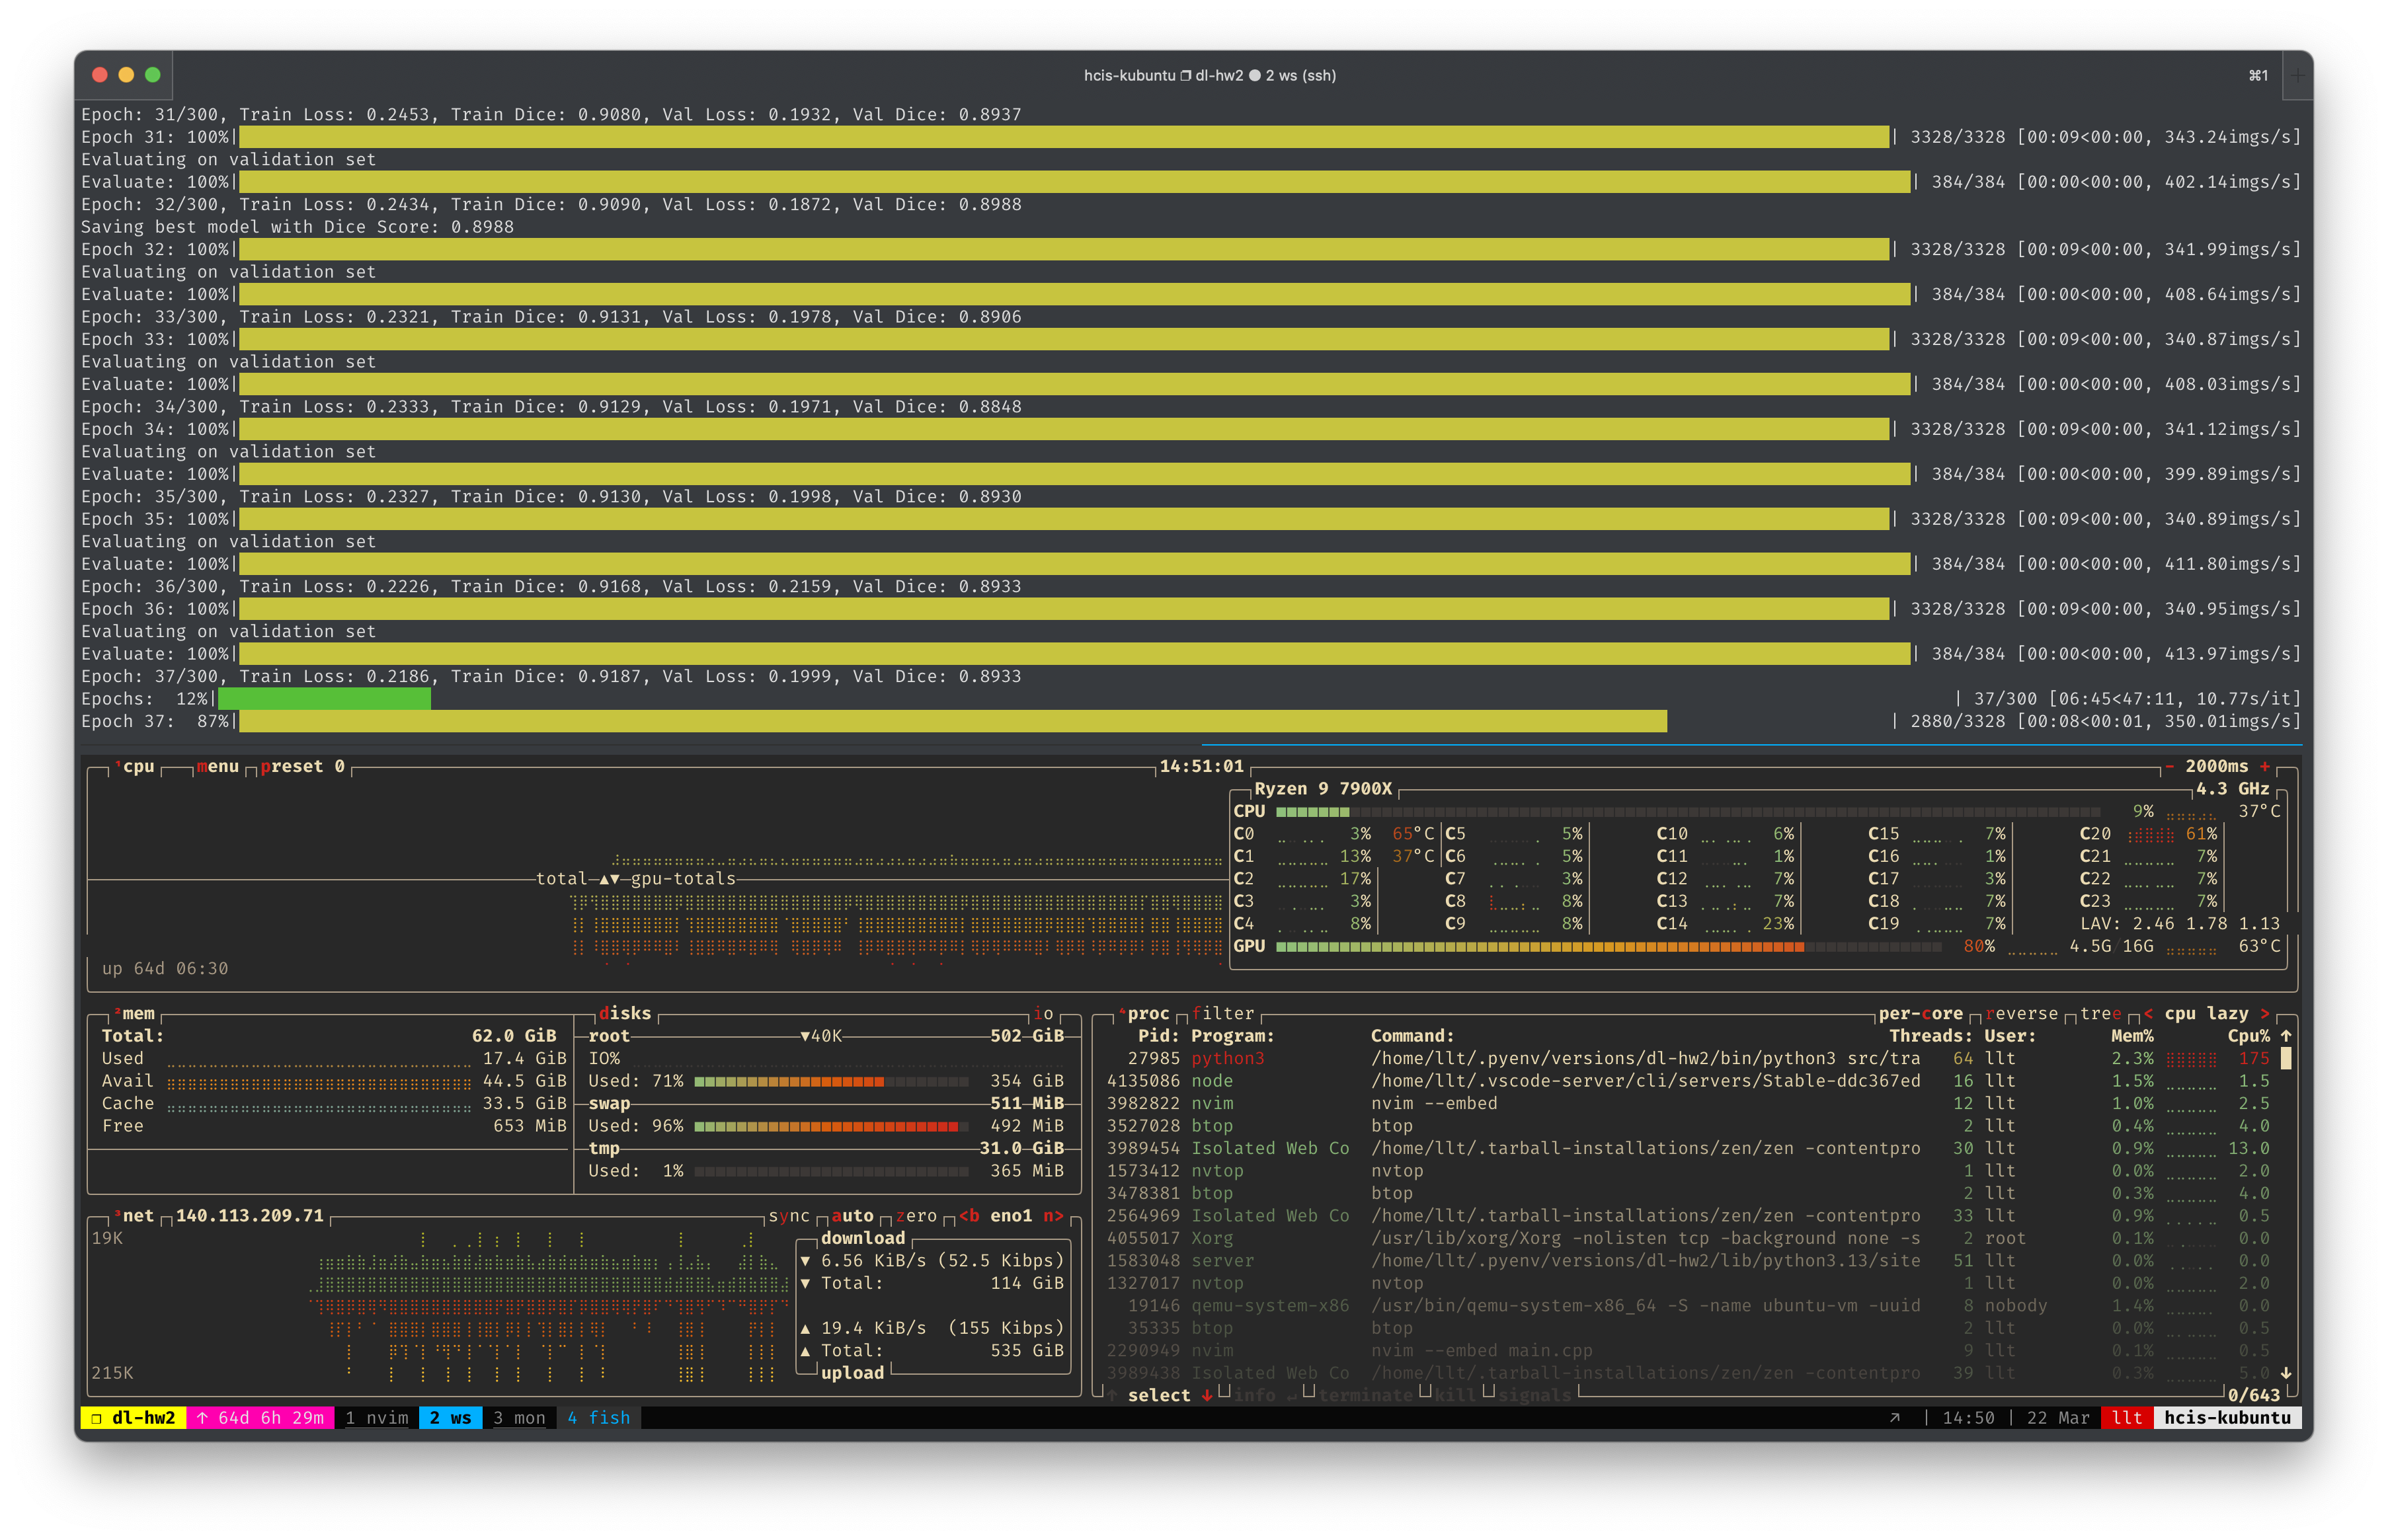
\includegraphics[width=0.8\textwidth]{./images/tqdm.png}
    \caption{The appearance of the progress bar, the terminal is splited using my configured \texttt{tmux} settings. And the bottom plane is a beautiful resouce monitor called \texttt{btop++}.}
    \label{fig:tqdm}
\end{figure}

\subsubsection{Report Figure Generation}

If you had seen the report of my last homework, you may notice that there are up to 10 tables different experiments' comparison.
And each of the table has 5 columns and 5 rows, that is 25 cells that need to be filled with the numbers.
I'm too lazy to fill the numbers manually, so I wrote some macros in the \LaTeX{} file to read the \texttt{accuracy.txt} file in the corresponding directory (according to the hyperparameters) and fill the numbers automatically.

And I also did somthing similar in this homework.
However, instead of inventing the wheels again, I used the \texttt{pgfplotstable} package to read the \texttt{epochs.csv} file and generate the figures automatically.
The \texttt{epochs.csv} file is generated by the \texttt{train.py} file, and it contains the training loss, validation loss, and validation Dice coefficient of each epoch.
The \texttt{pgfplotstable} package will read the \texttt{epochs.csv} file and generate the figures in the \LaTeX{} file.
All figures except Figure~\ref{fig:tqdm} in this report are generated by the \texttt{pgfplotstable} package.
You can see the \LaTeX{} source code for more details in both homeworks if you are interested.

Tl;dr, I used the \texttt{pgfplotstable} package to generate the figures in the report automatically instead of using \texttt{matplotlib} to generate the figures by another python script.


\section{Data Preprocessing}

For data preprocessing, I first resized the images to $256 \times 256$ pixels.
However, the model can perform very good while training on the training set but perform poorly on the validation set, which indicates that the model is overfitting and the model is not generalizing well.
Therefore, I started to consider using data augmentation to improve the generalization of the model.

\subsection{Data Augmentation}

After surveying many libraries, I found that the Albumentations library~\cite{Albumentations} is a very powerful library for image augmentation.
It is also suprised that the default code TA provided in \texttt{oxford\_pet.py} is very similar to the code in the official document of Albumentations.
Therefore, I decided to use Albumentations to augment the data.

The augmentation methods I used are as follows:

\begin{itemize}
    \item Resize: Resize the image to $256 \times 256$ pixels.
    \item HorizontalFlip: Flip the image horizontally.
    \item VerticalFlip: Flip the image vertically.
    \item Rotate: Rotate the image by an angle.
    \item RandomBrightnessContrast: Randomly change brightness and contrast of the image.
    \item HueSaturationValue: Randomly change hue, saturation and value of the image.
    \item RGBShift: Randomly shift values for each channel of the image.
    \item RandomGamma: Randomly change gamma of the image.
\end{itemize}

The augmentation methods are randomly applied to the images during training.
For testing and validation, only the resize operation is applied to the images.
This can prevent the model from overfitting and improve the generalization of the model.

The implementation of the transform using Albumentations is shown below:

\inputminted[firstline=158]{python}{../src/oxford_pet.py}


\section{Analyze and Experiment Results}
\subsection{Basic Experiment}

In the basic experiment, I used experimented two models on the Oxford-IIIT Pet dataset.

For both models, I used the following hyperparameters:
\begin{itemize}
    \item Batch size: 8
    \item Epochs: 100
    \item Optimizer: Adam
    \item Learning rate: $1 \times 10^{-4}$
    \item Scheduler: None
\end{itemize}


The training and validation dice score for both models are shown in Figure~\ref{fig:train_val_dice}.
The training and validation loss for both models are shown in Figure~\ref{fig:train_val_loss}.
We can see that both models have similar performance on the validation set, which has dice score higher than 0.9 on the validation set.
The training dice score is higher than the validation dice score, which is expected.
The training loss is lower than the validation loss, which is also expected.

\def \unetexpdir {../log/u1/}
\def \resunetexpdir {../log/ru1/}
\begin{figure}[ht]
    \centering
    \begin{tikzpicture}
        \begin{axis}[
                width=\linewidth,
                xlabel={Epoch},
                ylabel={Dice Score},
                % xmin=0,
                % xmax=100,
                height=0.5\linewidth,
                grid=major,
                title={Dice Score on Training/Validation Set},
                legend style={at={(0.98,0.02)},anchor=south east},
            ]
            \addplot table [
                    col sep=comma,
                    x=epoch,
                    y=val_dice,
                ]{\unetexpdir/epochs.csv};
            \addlegendentry{Unet (Validation)}
            \addplot table [
                    col sep=comma,
                    x=epoch,
                    y=val_dice,
                ]{\resunetexpdir/epochs.csv};
            \addlegendentry{ResUNet (Validation)}
            \addplot table [
                    col sep=comma,
                    x=epoch,
                    y=train_dice,
                ]{\unetexpdir/epochs.csv};
            \addlegendentry{Unet (Training)}
            \addplot table [
                    col sep=comma,
                    x=epoch,
                    y=train_dice,
                ]{\resunetexpdir/epochs.csv};
            \addlegendentry{ResUNet (Training)}
        \end{axis}
    \end{tikzpicture}
    \caption{Dice score on training and validation sets for both models}
    \label{fig:train_val_dice}
\end{figure}

\begin{figure}[ht]
    \centering
    \begin{tikzpicture}
        \begin{axis}[
                width=\linewidth,
                xlabel={Epoch},
                ylabel={Loss},
                % xmin=0,
                % xmax=100,
                height=0.5\linewidth,
                grid=major,
                title={Loss on Training/Validation Set},
                % legend style={at={(1,1)},anchor=north east},
            ]
            \addplot table [
                    col sep=comma,
                    x=epoch,
                    y=val_loss,
                ]{\unetexpdir/epochs.csv};
            \addlegendentry{Unet (Validation)}
            \addplot table [
                    col sep=comma,
                    x=epoch,
                    y=val_loss,
                ]{\resunetexpdir/epochs.csv};
            \addlegendentry{ResUNet (Validation)}
            \addplot table [
                    col sep=comma,
                    x=epoch,
                    y=train_loss,
                ]{\unetexpdir/epochs.csv};
            \addlegendentry{Unet (Training)}
            \addplot table [
                    col sep=comma,
                    x=epoch,
                    y=train_loss,
                ]{\resunetexpdir/epochs.csv};
            \addlegendentry{ResUNet (Training)}
        \end{axis}
    \end{tikzpicture}
    \caption{Loss on training and validation sets for both models}
    \label{fig:train_val_loss}
\end{figure}


\section{Execution Steps}
\subsection{Training}

For training the UNet model, you can use the following command:

\begin{minted}{bash}
python3 src/train.py -b 8 -e 200 -o u1 -lr 0.0001 -m unet
\end{minted}

The command above will train the model with a batch size of 8, 200 epochs, Adam optimizer (by default), and a learning rate of $1 \times 10^{-4}$.

For training the ResUNet model, you can use the following command:

\begin{minted}{bash}
python3 src/train.py -b 8 -e 200 -o ru1 -lr 0.0001 -m resunet
\end{minted}

Note that the \texttt{-o} option is used to specify the output directory for saving the model and logs. You can change the output directory to any directory you want.
But mentioned that the output directory should will be prefixed with \texttt{log/}.

\subsection{Inference}

For inference, you can use the following command:

\begin{minted}{bash}
python3 src/inference.py -m unet -o u1 -w best_model.pth
python3 src/inference.py -m resunet -o ru1 -w best_model.pth
\end{minted}


\section{Discussion}
\subsection{Double Convolution Without Batch Normalization}

Since the UNet model I implemented use the double convolution block with batch normalization that Olaf Ronneberger et al.~\cite{UNet} didn't use, I decided to implement the double convolution block without batch normalization to see how it affects the performance of the model.

The result of the model with double convolution block without batch normalization is shown in Figure~\ref{fig:train_val_dice_wo_bn} and Figure~\ref{fig:train_val_loss_wo_bn}.

\comparisonfigures{wo_bn}{Without Batch Normalization}

We can see that the model with double convolution block without batch normalization has a slightly lower performance than the model with batch normalization.

\subsection{DyT: Replace Batch Normalization with DyT}
\label{sec:dyt}

However, the double convolution block without batch normalization is not the only way to replace batch normalization.
Jiachen Zhu et al.~\cite{DyT} proposed that Transformers without normalization can achieve similar or even better performance with a remakably simple technique called DyT.
DyT is a simple technique that replaces the normalization layer with parameterized tanh (Dynamic Tanh), which is an element-wise operation that scales the input tensor by a learnable parameter.

The implementation of DyT is quite simple, it is shown below:

\inputminted[firstline=5, lastline=20]{python}{../src/models/common.py}

The result of the model with DyT is shown in Figure~\ref{fig:train_val_dice_dyt2d} and Figure~\ref{fig:train_val_loss_dyt2d}.
We can see that the model with DyT has a similar performance to the model without batch normalization, which is slightly lower than the model with batch normalization, but still have a dice score higher than 0.9 on the validation set for the last few epochs.
And the figure also shows that it is even not as stable as the model without batch normalization.

This might be because the DyT is not suitable for the double convolution block, since it is designed for the Transformer model.
It is worth to investigate more on why DyT doesn't work well on the double convolution block and how to replace the batch normalization layer with DyT in the double convolution block.

\comparisonfigures{dyt2d}{Replace Batch Normalization with DyT2d}


\printbibliography

\end{document}
